\documentclass[IN,11pt,twoside,openright,idp,english]{tumthesis}

\usepackage[backend=bibtex,style=ieee]{biblatex}
\usepackage{xcolor}
\usepackage{amsmath}
\usepackage{booktabs}
\usepackage{listings}
\lstset{numbers=none,basicstyle=\footnotesize\ttfamily,breaklines=true}
\usepackage{url}
\usepackage[style=base]{caption}
\captionsetup[subfloat]{font={rm,footnotesize},labelfont={rm}}	
\usepackage[hang]{footmisc}
\setlength\footnotemargin{5pt}

\titleenglish{Development of a Framework for Retrieval of Parameters of the Starlink Dish}
\titlegerman{Entwurf eines Frameworks zur Informationsgewinnung von Parametern der Starlink Dish}
\author{Roberto Castellotti}
\supervisor{\chairhead}
\assistants{Leander Seidlitz, Johannes Zirngibl}
\advisor{Leander Seidlitz, Johannes Zirngibl}
\courseofstudy{Informatics}
\date{September 15, 2016}
\location{Garching}
\setcounter{tocdepth}{2}
\addbibresource{ref.bib}

\begin{document}
\pagenumbering{gobble}	
\maketitle
\cleardoublepage

\begin{abstract} 
In this report, we document our work and findings on Starlink-based connections. 

After introducing the principles behind Low Earth Orbiting satellites Internet connection and introducing technologies to work on satellites, we investigated whether Starlink-based connections result in a different routing of packets when reaching geographically sparse targets; we moved then to analyzing whether the dish performs some buffering before relaying packets to the satellite.

Lastly, we analyzed satellites visible from a dish and, after developing a script to detect satellite handovers, we moved on to trying to correlate drops in bandwidth and satellite handovers; handovers do not seem to happen in a specific pattern, nor are indicative of a drop in bandwidth, this means the connection is very stable from an end-user perspective.

While performing our research, we developed tooling to interact with the dish and run measurements.
\end{abstract}

\tableofcontents
\listoffigures
\listoftables
\startcontent
\chapter{Introduction and Background}

\section{Introduction}

Starlink \footnote{\url{https://www.starlink.com/}} is the largest Low Earth Orbiting, hereinafter LEO, satellite constellation. SpaceX manages it, and its scope is to bring Internet broadband connection in the most remote and rural areas in the world while also serving people living in residential areas, who would typically use a cabled link.

LEO satellites orbit around 550 kilometers from Earth, so naturally, LEO connections have a lower latency than other satellite-based connections. SpaceX claims latency is around ~25 ms. Our experiments showed that it is often higher (~45ms). 

Starlink might not be the best solution for people living in residential areas, as their place is covered by a faster cabled connection, probably way cheaper as the infrastructure is more straightforward to maintain. As of October 2023, Starlink costs 65 USD per month with a one-time hardware cost of 450 USD. 

Satellite-based Internet connections have been around for several years. They are based on geostationary satellites, hereinafter GEOSAT, orbiting at about 35.000 kilometers; it is thus natural to expect higher latency when comparing GEOSAT connections to cabled Internet connections; we are talking about around 600 ms for latency, or in other words, Starlink averages ~70 RTTs in the time a GEOSAT satellite does 1 RTT.

From a customer perspective, using Starlink is straightforward; after receiving his hardware package, he only needs to plug the satellite dish he receives (see Figure \ref{fig:dish}) and position it in a place with clear access to the sky. After that, plugging in the router is enough to start browsing the Internet.

On a more technical note, what is happening to packets sent from a local device is they go through the dish, they are relayed to a nearby satellite, and they are sent to a ground station in view; from that point onwards, packets are routed normally through the Internet.

SpaceX also experiments with Inter Satellite Links, allowing satellites to communicate without resorting to local ground stations. This is crucial for the maritime version of the Starlink kit. Moreover, it might be possible that using laser links is faster than fiber on Earth, thus providing lower latency connection to everyone, as reported by Elon Musk himself \cite{tweet}.

\begin{figure}
  \centering
  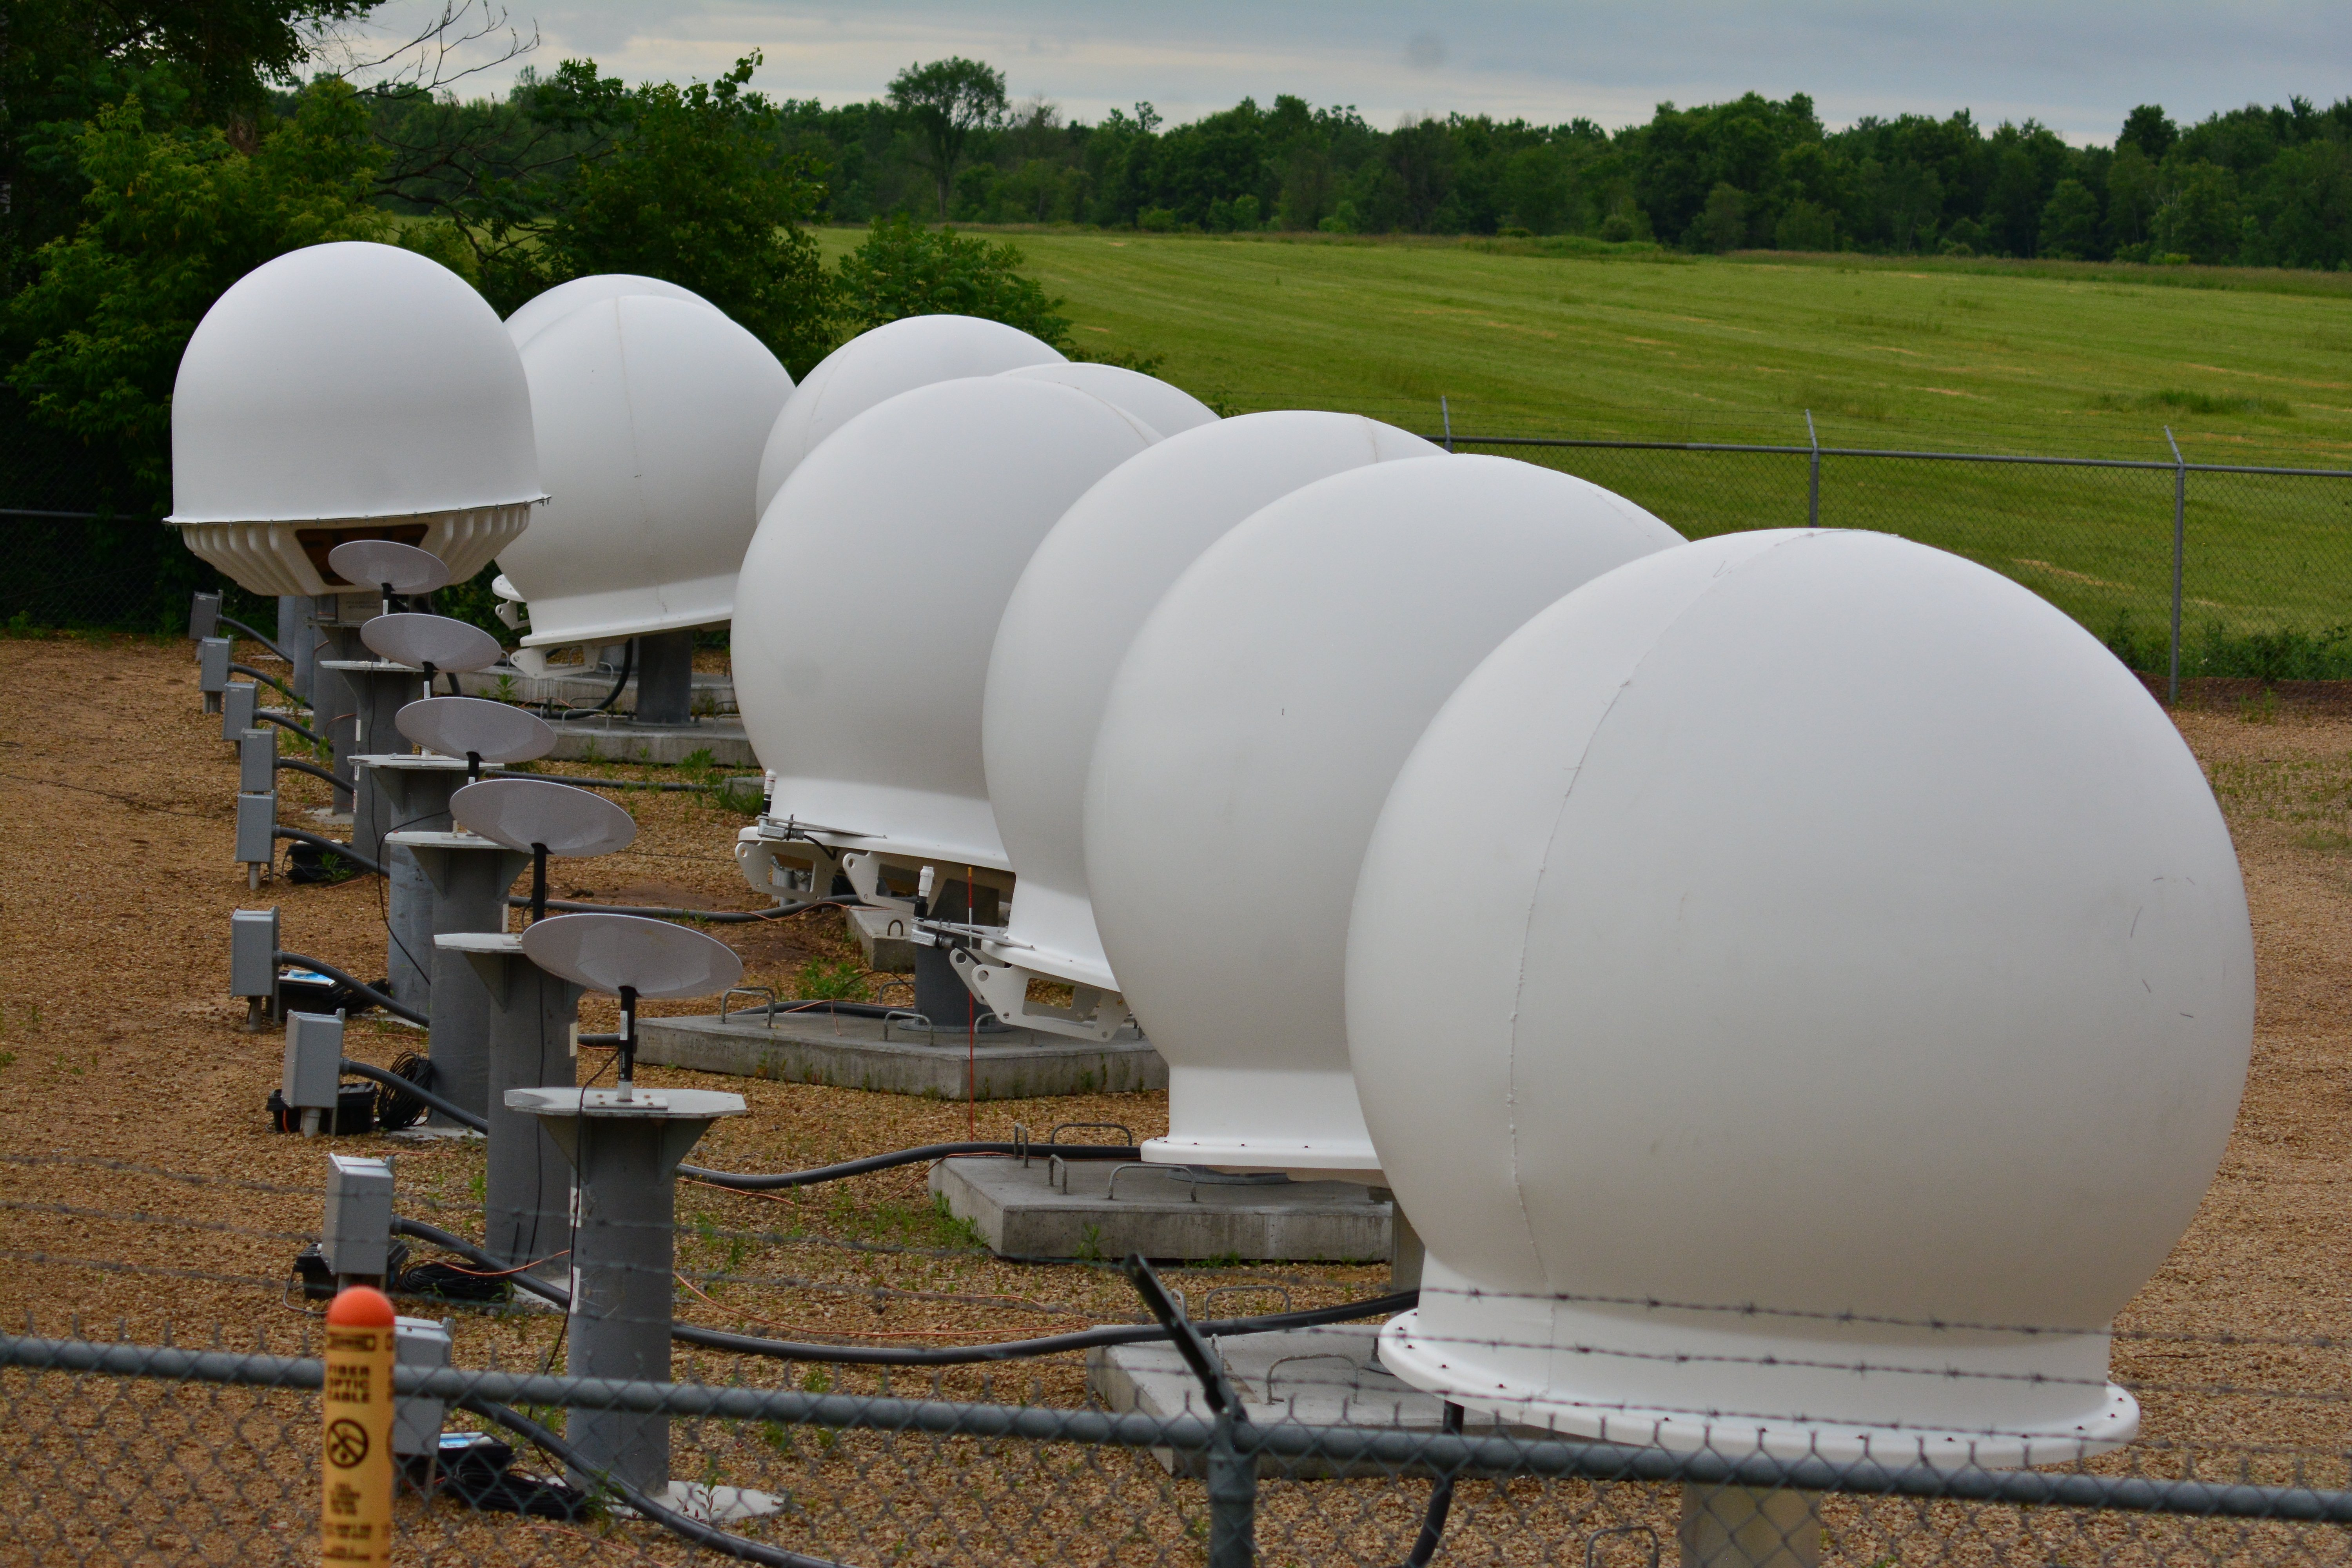
\includegraphics[width=0.6\columnwidth]{img/ground-station.jpeg}
  \caption{A sample ground station, from \protect\url{https://www.reddit.com/r/SpaceXLounge/comments/hcf4t5/prototype_starlink_terminal_closeups_merrillan_wi/}}
  \label{fig:gs}
\end{figure}

\begin{figure}
  \centering
  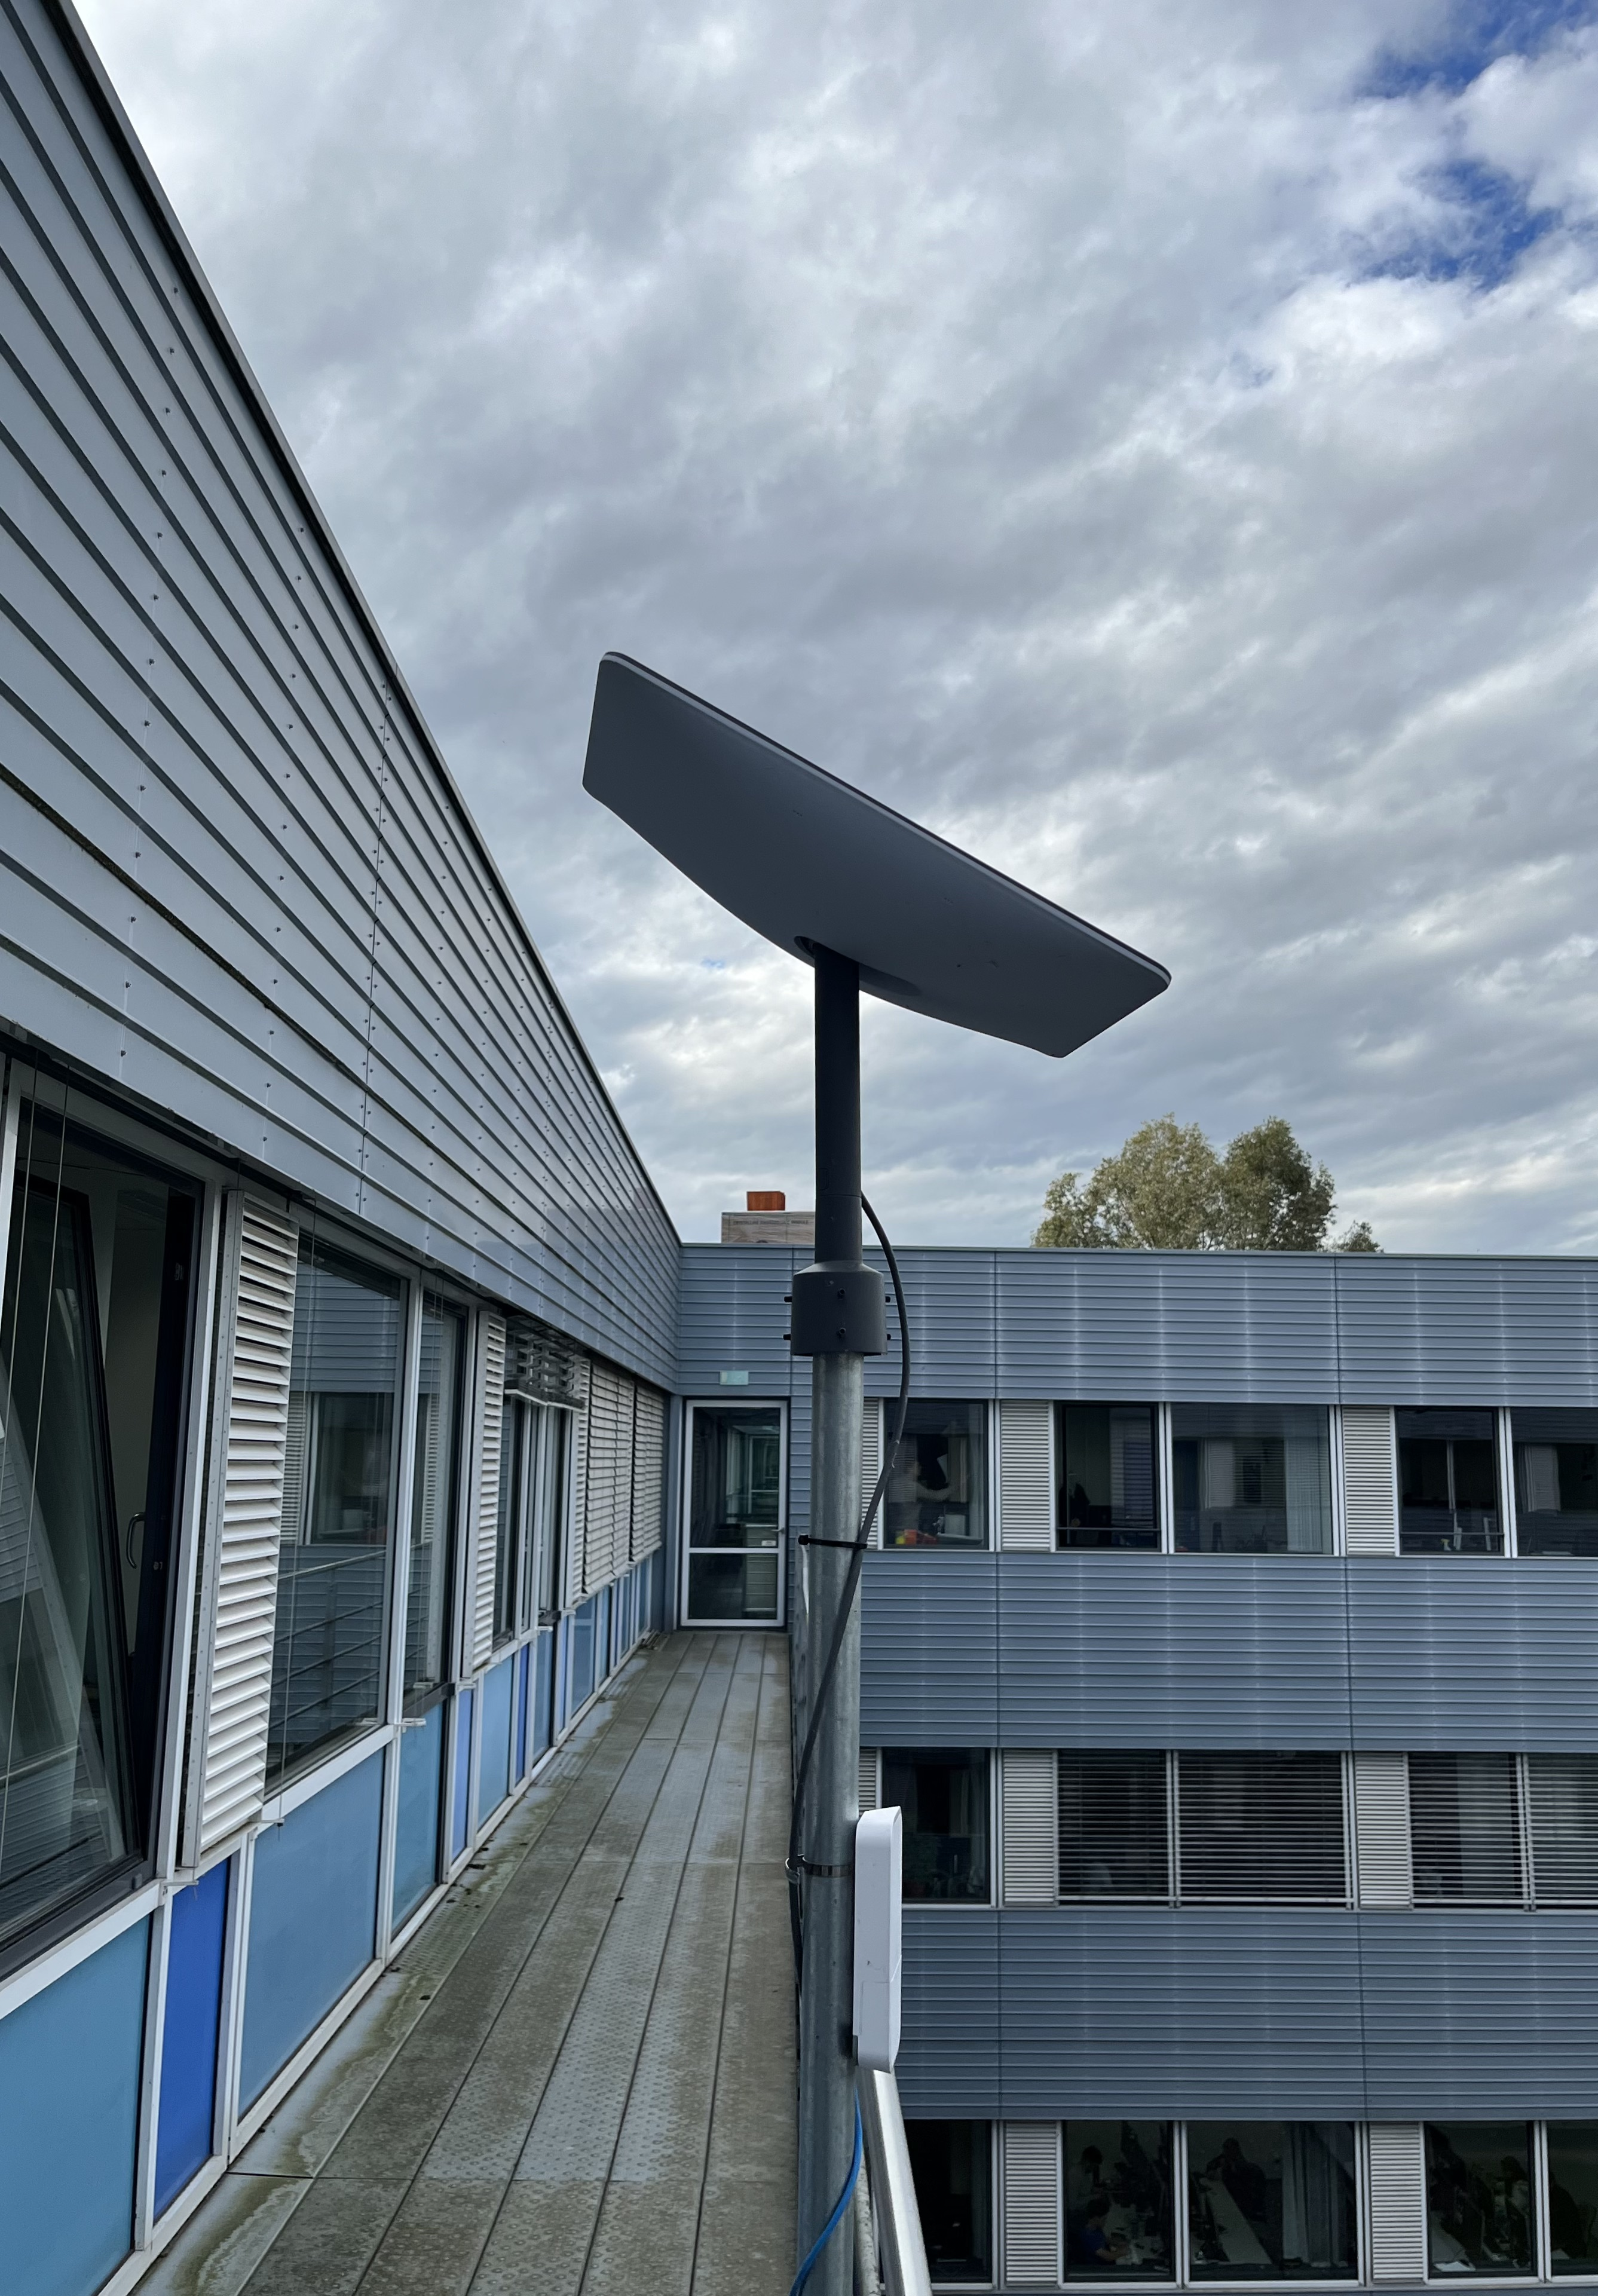
\includegraphics[width=0.6\columnwidth]{img/dish.jpeg}
  \caption{Starlink dish, picture from  \protect\url{https://www.starlink.com/technology}}
  \label{fig:dish}
\end{figure}

\begin{figure}
  \centering
  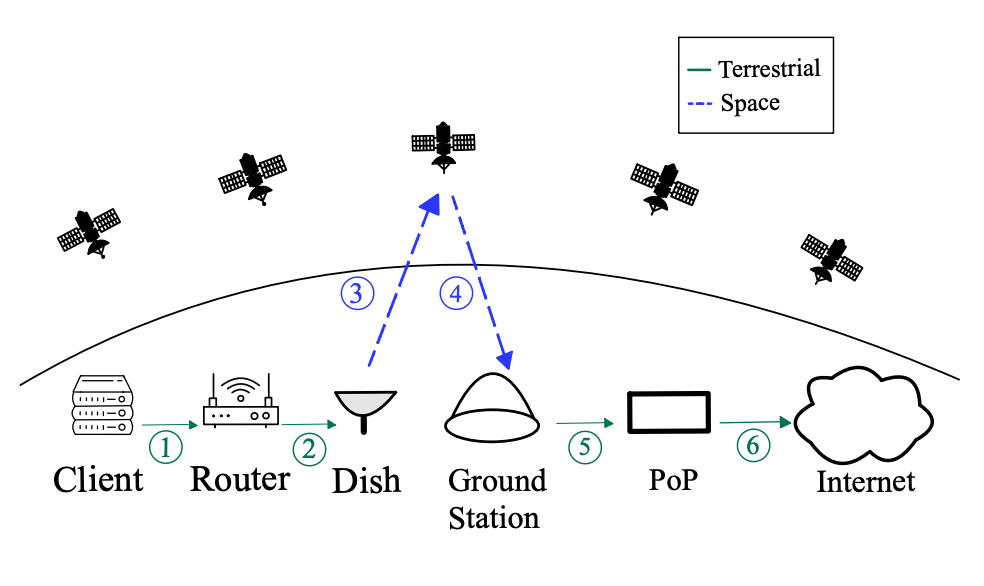
\includegraphics[width=0.6\columnwidth]{img/starlink-101.png}
  \caption{Basic Starlink working, from \cite{izhikevich2023democratizing}}
  \label{fig:starlink-101}
\end{figure}

SpaceX is currently the most popular LEO-based Internet Service Provider. However, other similar projects exist, such as OneWeb \footnote{https://oneweb.net/} and Amazon Project Kuiper \footnote{https://www.aboutamazon.com/what-we-do/devices-services/project-kuiper}. The former one is more enterprise and government-focused. At the same time, Project Kuiper aims to compete with Starlink, effectively commercializing a similar product. The future is bright for LEO-based ISPs!

\section{Background}

We will now introduce some concepts we will use later. First, let us describe Two Line Element Sets, the data format to encode the position of satellites.

\subsection{Two-line Element Sets}

Two-line Element Sets (hereinafter TLEs) is a widely used ASCII-based data format to encode the position of orbital elements for a given point in time \footnote{\url{https://en.wikipedia.org/wiki/Two-line_element_set}}. We will be working with TLEs using the Skyfield Library, \footnote{\url{https://rhodesmill.org/skyfield/}}, an elegant astronomy library for Python. Check Appendix \ref{app:sky} for a sample script to localize a satellite's position given the Satellite Name. A complete list of Starlink satellite names can be found at \url{https://celestrak.org/NORAD/elements/gp.php?GROUP=starlink}. SATNAME is a unique identifier.

Knowing the position of a satellite at any given time allows us to restrict the subset of satellites the dish may be connected to; it is worth noting that previously, it was possible to call the \texttt{dish\_get\_context} or similar methods to retrieve such information. Unfortunately, these methods either return a \texttt{PermissionDenied} error or are deprecated.

\begin{lstlisting}[caption={TLE for satellite STARLINK-1007 },captionpos=b]
STARLINK-1007           
1 44713U 19074A   23239.65120160  .00022666  00000+0  15354-2 0  9991
2 44713  53.0553  19.2809 0001296  68.3392 291.7735 15.06406564209327
\end{lstlisting}

\subsection{Visible Satellites}
% It is up to us to define what "visible" means, in our evaluations we decided that, knowing the satellites orbit around the earth at around 550 kms in height it is reasonable to assume a satellite is visible when it is above the horizon and it is (point to point) not further than 800 kms. The ground truth might be different, but this approximation allows us to approximately have an idea about what is going on in space. 

% The first measurement we are setting up is the following: every 15 seconds we run a script that gets all the "visible" satellites and we store them in a SQLite database, if we see the same satellite in the iteration before we simply update the \texttt{timestamp}, otherwise we create a new row in the db. We use a \texttt{relative\_ts} (relative timestamp) to enumerate every measurement (a probe every 15 seconds). To measure visible satellites we are running the following command: \texttt{python3 visible-satellites.py -v -lat 48.2489 -lon 11.6532 -el 0 -d 800}, where \texttt{lat} and \texttt{lon} are Garching's coordinates, we are not interested in using an elevation.


\subsection{Patterns in Satellites Appearances}
% After having collected data for several hours we decided to plot satellite appearances to check whether they were following some patterns, it seems like it is the case, as you can see in Figure \ref{fig:vis-sat-pat}. We see the same satellite each 12 hours roughly, for some satellites we notice something that might seem like a change in the pattern, but this is not really true, the interval between the appearances is the same as in the other cases, we are not sure we understand why we are seeing this artifact.

% \begin{figure}
% 	\centering
% 	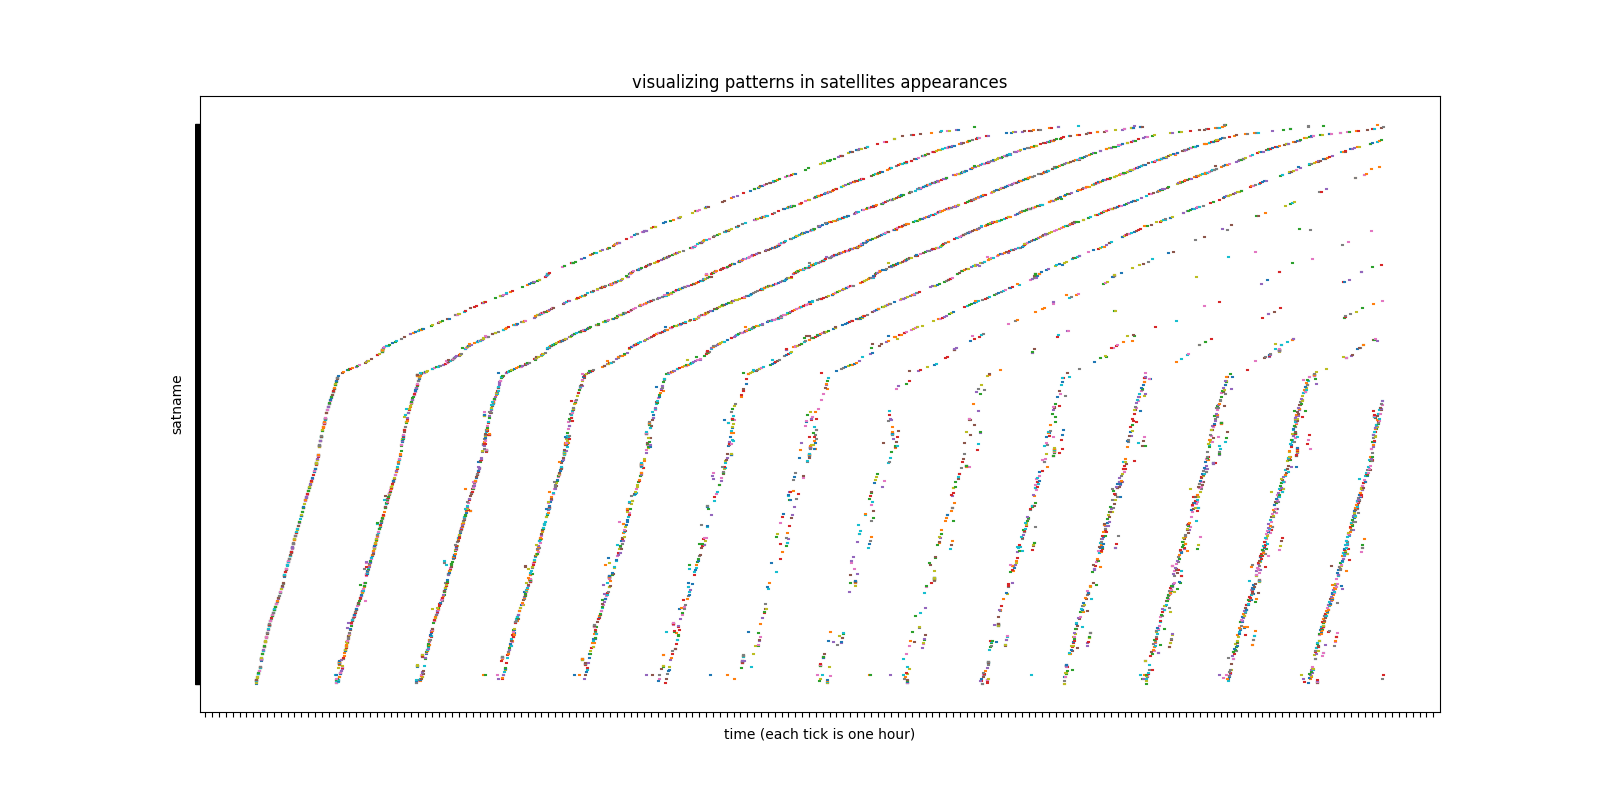
\includegraphics[width=1.2\columnwidth]{img/visualizing-how-long-satellites-are-visible-for.png}
% 	\caption{Visualizing patterns in satellite appearances, we roughly see the same satellite each 12 hours.}
% 	\label{fig:vis-sat-pat}
% \end{figure}

  
\section{Related work}

Being Starlink a novel technology the existing body of research is somewhat limited, but papers and tools \footnote{https://github.com/danopstech/starlink\_exporter}, \footnote{https://github.com/sparky8512/starlink-grpc-tools} are in development, we created some scripts to work with the dish and to perform some measurements, you can find them in the very same repository that contains this report \footnote{https://gitlab.lrz.de/netintum/teaching/tumi8-theses/idp-castellotti}.

From a research perspective, different works provide more insights into Starlink. Papers like \cite{pan2023measuring} focus on describing the infrastructure Starlink uses. In contrast, \cite{izhikevich2023democratizing} illustrates a novel approach to make measurements simpler and cheaper, and \cite{browser-side} focuses on running some client-side measurements with a browser extension.

Some work was recently on the hardware side, like \cite{glitching} while \cite{quarkslab} focuses on the firmware perspective and gives some insight into the gRPC API.


% Maybe this should be environment?

Our setup is pretty simple; the machine we use to run measurements and use the Starlink connection is directly connected to the dish.

Our first approach to the dish was through the web UI reachable at 192.168.100.1; we discovered it is getting data from a gRPC API running directly on the dish, so we decided to spend some time documenting the available methods we could later use to gather useful additional information.

A server-reflected \footnote{\url{https://github.com/grpc/grpc/blob/master/doc/server-reflection.md}} gRPC
\footnote{\url{https://grpc.io}} API is running on the dish; we can access it by querying it at \texttt{192.168.100.1:9200} using a tool like grpcurl \footnote{\url{https://github.com/fullstorydev/grpcurl}}, a sample query to retrieve downlink throughput is:

\begin{lstlisting}[language=bash,basicstyle=\tiny]
grpcurl -plaintext -d '{"get_status":{}}' 192.168.100.1:9200 SpaceX.API.Device.Device/Handle
\end{lstlisting}

It is then possible to use \texttt{jq} to extract the needed fields. We can use the following command to describe the available services:

\begin{lstlisting}[language=bash,basicstyle=\tiny]
rc@gnolmir ~> grpcurl -plaintext 192.168.100.1:9200 describe
SpaceX.API.Device.Device is a service:
service Device {
	RPC Handle ( .SpaceX.API.Device.Request ) returns ( .SpaceX.API.Device.Response );
	...
}
\end{lstlisting}

And then describe the service using:

\begin{lstlisting}[language=bash,basicstyle=\tiny]
grpcurl -plaintext 192.168.100.1:9200 describe SpaceX.API.Device.Request
\end{lstlisting}

A complete list of available methods as of September 2023 can be found in the Appendix Section \ref{starlink-grpc}

To simplify scripting, we developed a very simple wrapper library around the gRPC API  \footnote{\url{https://gitlab.lrz.de/netintum/teaching/tumi8-theses/idp-castellotti/-/blob/main/nine981.py}} and a CLI tool \footnote{\url{https://gitlab.lrz.de/netintum/teaching/tumi8-theses/idp-castellotti/-/blob/main/s.py}} to use the library in command line. It should be trivial to add functionality to the library, unlike \texttt{sparky8512/starlink-grpc-tools}, we decided not to make any assumption about the format data is saved in.


\chapter{Measurements}

introuduce the kind of measurements we will run

\section{Routing}


% One of the first experiments we performed was running traceroutes to several different geographically sparse targets, we retrieved a list of those from major cloud vendors, \footnote{\url{ https://www.gstatic.com/ipranges/cloud.json}}, \footnote{\url{https://ip-ranges.amazonaws.com/ip-ranges.json}, \url{https://www.microsoft.com/en-us/download/details.aspx?id=53601}, \url{https://docs.oracle.com/en-us/iaas/tools/public_ip_ranges.json }}, since we approximately know the location of the hosts, even though we can never be sure the last target we reach with a traceroute in complex networks reflects the position of the target we were trying to reach, it is completely possible we hit a load balancer of we enter a private network and loose track of our packets afterwards.

% We ran the traceroutes using ICMP, UDP and TCP using both the Starlink and the default network interface over several days to see whether we can spot some differences when visualizing them using NetworkX, a Python package for the creation, manipulation, and study of the structure, dynamics, and functions of complex networks. \footnote{\url{https://networkx.org/}}. We are limiting ourselves to the first 7 hops because we don't receive answers for any further hops. 

% \begin{figure}
% 	\label{fig:tr_aws_icmp}
% 	\centering
% 	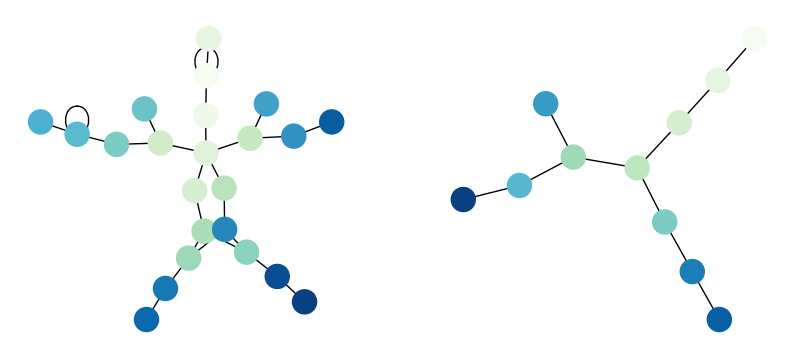
\includegraphics[width=0.6\columnwidth]{img/tr_aws_icmp.png}
% 	\caption{Visualizing traceroutes to 4 different hosts from AWS using ICMP, left figure refers to Starlink traceroutes, right one is default network interface.}
% \end{figure}

% \begin{figure}
% 	\label{fig:tr_aws_udp}
% 	\centering
% 	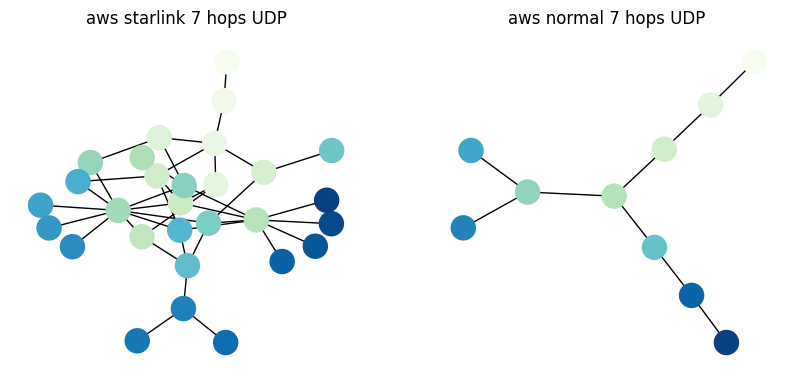
\includegraphics[width=0.6\columnwidth]{img/tr_aws_udp.png}
% 	\caption{Visualizing traceroutes to 4 different hosts from AWS using UDP, left figure refers to Starlink traceroutes, right one is default network interface.}
% \end{figure}

% \begin{figure}
% 	\label{fig:tr_aws_tcp}
% 	\centering
% 	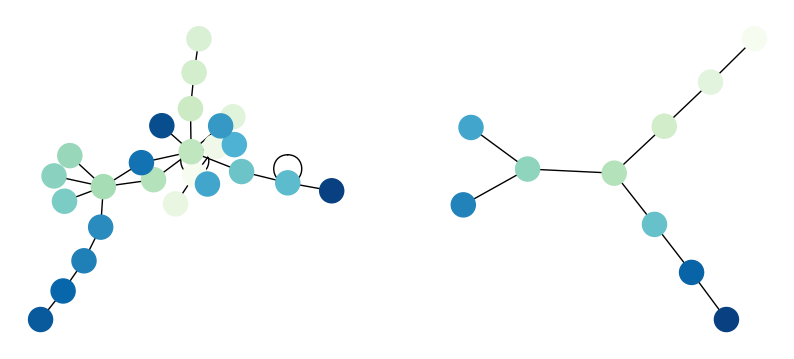
\includegraphics[width=0.6\columnwidth]{img/tr_aws_tcp.png}
% 	\caption{Visualizing traceroutes to 4 different hosts from AWS using TCP, left figure refers to Starlink traceroutes, right one is default network interface.}
% \end{figure}

% \begin{figure}
% 	\label{fig:tr_azure_icmp}
% 	\centering
% 	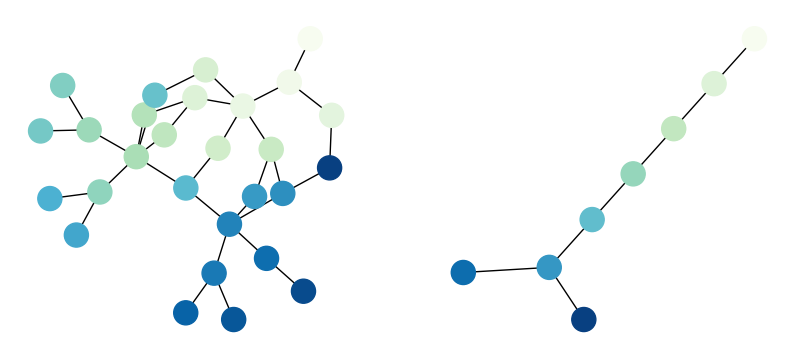
\includegraphics[width=0.6\columnwidth]{img/tr_azure_icmp.png}
% 	\caption{Visualizing traceroutes to 4 different hosts from Azure using ICMP, left figure refers to Starlink traceroutes, right one is default network interface.}
% \end{figure}

% Traceroutes don't tell us a lot, with a minor exception: we note that routing in Starlink is way more complex, in the "default" traceroutes we see traffic going to 4 different main directions, while it is much more garbled in the Starlink case. We are only reporting traceroutes to AWS using the three most common methods and a traceroute to Azure, more data to visualize can be found in the accompanying repository. \footnote{\url{https://gitlab.lrz.de/netintum/teaching/tumi8-theses/idp-castellotti-data}}

% We didn't find any significant differences comparing traceroutes over different days, we see hops in the same Autonomous Systems, the only difference we were able to observe is we reach different hosts inside AS 14593, the Autonomous System SpaceX operates, \footnote{\url{https://bgp.he.net/AS14593}}, the following is a table of hosts reached toghether along with a count of how many times we reached the target.

% \begin{table}[]
% 	\centering
% 	\begin{tabular}{ r r }
% 		\toprule
% 		host           & count \\ 
% 		\midrule
% 		206.224.65.204 & 595   \\
% 		206.224.65.200 & 595   \\
% 		206.224.65.208 & 549   \\ 
% 		206.224.65.182 & 444   \\
% 		206.224.65.196 & 440   \\ 
% 		206.224.65.188 & 360   \\ 
% 		206.224.65.129 & 358   \\ 
% 		206.224.65.178 & 274   \\ 
% 		206.224.65.180 & 235   \\ 
% 		206.224.65.184 & 189   \\ 
% 		206.224.65.186 & 159   \\ 
% 		206.224.65.190 & 151   \\
% 		\bottomrule
% 	\end{tabular}
% 	\caption{Targets reached inside AS14593 toghether with the count}
% 	\end{table}

% It is worth noting we also see some different prefixes in later traceroutes, AS14593 advertises a lot of them, the previous table is just a snapshot at a given moment.


\section{Latency Analysis}
% Since we have a way to extract a \texttt{pop\_ping\_latency\_ms} from the gRPC api we decided to measure the latency to the Pop (Point of Presence), we assume PoPs are physically near ground stations, but we are not entirely sure, in AS14593 we know there are several hosts distributed geographically containing "pop" in their hostname, such as \texttt{customer.dnvrcox1.pop.starlinkisp.net} 
% \footnote{\url{https://gitlab.lrz.de/netintum/teaching/tumi8-theses/idp-castellotti-data/-/blob/main/pops.json}}.

% Latency to the PoP is pretty stable, as SpaceX reports it fluctuates around 30 ms, as we can verify from Figure \ref{fig:vis-latency}, we weren't able to detect any patterns in latency fluctuation.

% \begin{figure}
% 	\centering
% 	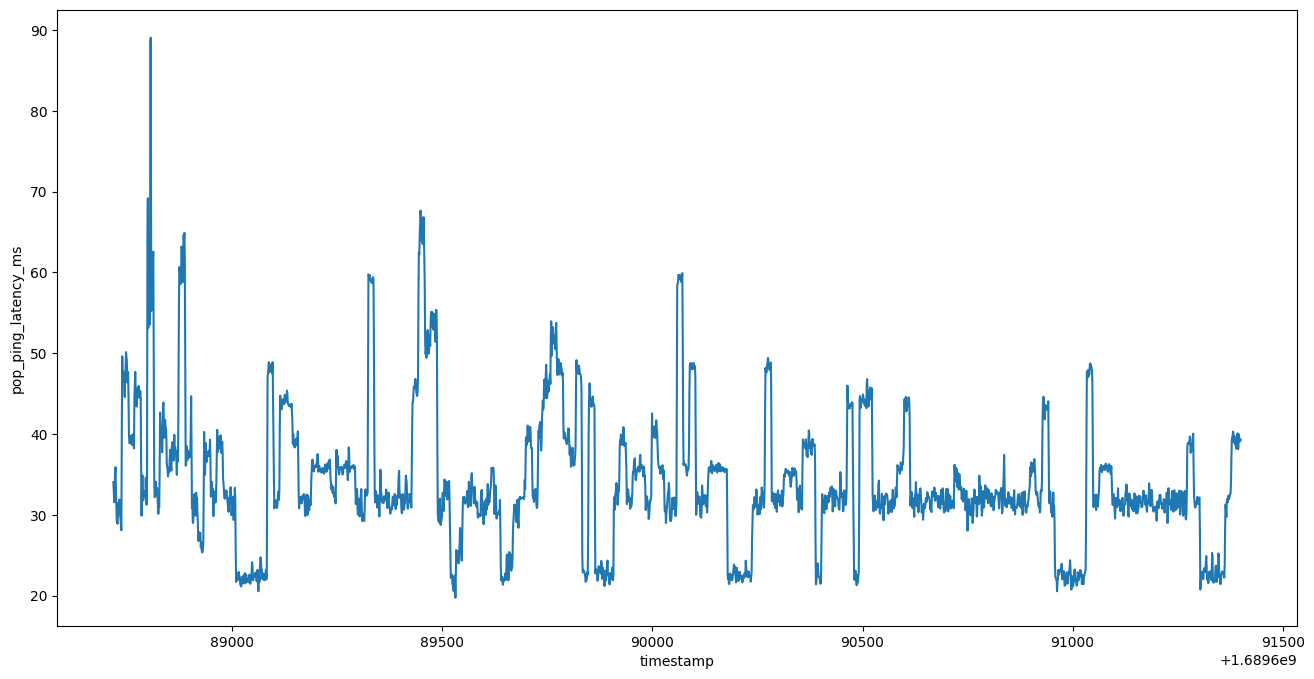
\includegraphics[width=1\columnwidth]{img/latency.png}
% 	\caption{Visualizing latency to the Point of Presence.}
% 	\label{fig:vis-latency}
% \end{figure}

\section{Bandwidth analysis}
% During our investigations we decided to analyze bandwidth for two reasons: first one first is we wanted to check wheter the data from the API was correct and then we also planned to investigate whether we could detect any patterns in bandwidth drops.

% The first experiment we set up was the following: we started downloading 5 debian ISOs from different mirrors (to neutralize the effect of the single upload speed of a mirror) while running a script to extract downlink throughput from the dish while also measuring it, simply by getting data from \texttt{/sys/class/net/{interface}/statistics/rx\_bytes}.

% As reported in Figure \ref{fig:vis-bw-15sec} we can see the dish reports throughput correctly.

% From \cite{llc-application} we know the dish is seeking for better connections, as satellites move constantly each 15 seconds. We plotted the data and tried to verify whether we could notice some phenomenon correlated to these 15 seconds intervals.

% \begin{figure}
% 	\centering
% 	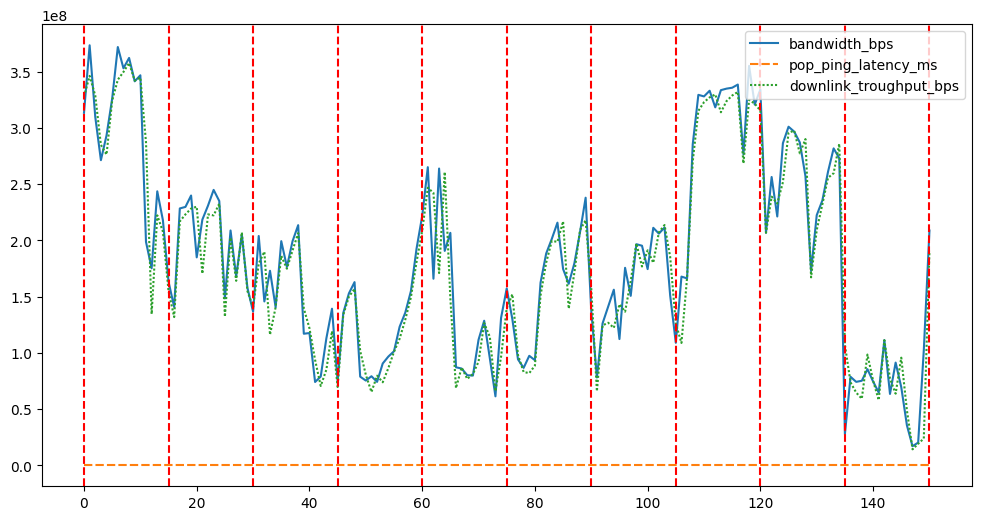
\includegraphics[width=1\columnwidth]{img/bw-15seconds.png}
% 	\caption{Visualizing bandwidth, \texttt{bandwidth\_bps} is the data we obtain from \texttt{/sys/class/net/{interface}/statistics/rx\_bytes}, while \texttt{downlink\_throughput\_bps} is the data reported from the gRPC api. Additionally we are drawing a vertical red line each 15 seconds.}
% 	\label{fig:vis-bw-15sec}
% \end{figure}

% We repeated the experiments shifting the red vertical lines and changing the intervals for collected data, and in the majority of cases we saw that whenever we drew a vertical red line we had some drop in the immediate milliseconds before or after, however drops also happen in different intervals. We thought it was possible these drops where somewhat related to satellite handovers, so we decided to further investigate.  







\section{Physical layer influences on latency}

% After measuring latency and bandwidth in \ref{sec:bw} and noticing some drops in semi-regular intervals we decided to investigate whether the dish was buffering packets in some way, our intuition is that if this is the case we can approximately detect the buffer size, this means in the best-case scenario we send the packet we want to reach the Internet exactly, it fills the buffer and it is sent immediately.

% To verify whether this hypotesis was true we tried to send some payload with iPerf \footnote{\url{https://iperf.fr/}} on the network interface used by Starlink, we sent payload of increasing sizes (10k, 20k, 50k, 100k, 1M, 10M)) and we measured the RTT, the following is a visualization, as we can notice sending some traffic does not have an impact.

% \begin{figure}
% 	\centering
% 	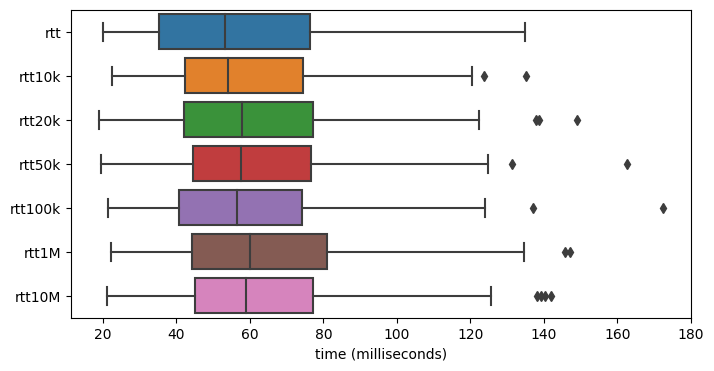
\includegraphics[width=0.6\columnwidth]{img/latency_iperf.png}
% 	\caption{Latency variation while sending traffic on the uplink using iPerf}
% \end{figure}

\section{Detecting Satellite Handovers}

% Unfortunately,as mentioned it is not anymore possible to know from the gRPC API which satellite the dish is connected, it used to be possible during the pre-beta phase \footnote{\url{https://www.reddit.com/r/Starlink/comments/p84o5i/comment/h9o1elp/}}.
% The Starlink gRPC api exposes a \texttt{dish\_get\_obstruction\_map} method, following the approach described in \cite{izhikevich2023democratizing} we use the information gathered from polling the endpoint each second to extract the current obstruction map and visualize satellite handovers. The reason this works is the dish is adding a dot (setting a value to 1) in a 123*123 matrix whenever it sees a satellite in that position. Whenever the dish is rebooted (using i.e \texttt{nine981.reboot}) the matrix is cleared by setting every entry to -1, whenever a satellite is detected the entry is set. By polling the endpoint frequently enough we can observe satellites traces, by comparing values in the matrices we obtain we can detect whether a satellite handover was performed.

% \begin{figure}	
% 	\centering
% 	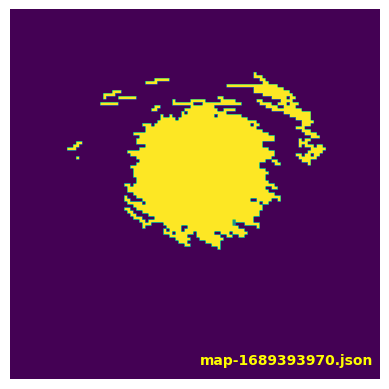
\includegraphics[]{img/obstruction_map_finale.png}
% 	\caption{An obstruction map retrieved by the dish}
% \end{figure}


% Let's assume the two following matrices are retrieved at $ t_x $ and $ t_{x+1} $ respectively. In the first matrix we have ones in $ (0,2) $ and $ (1,3) $, in the second one we have ones in $ (0,2) $, $ (1,3) $, $ (2,4) $, this means the new satellite we saw at $ t_{x+1} $ is on the same path as the satellites before, thus NO handover was not performed.
% \[
% \begin{bmatrix}
% -1 & -1 & \color{red}1 & -1 & -1 \\
% -1 & -1 & -1 & \color{red}1 & -1 \\
% -1 & -1 & -1 & -1 & -1 \\
% -1 & -1 & -1 & -1 & -1 \\
% -1 & -1 & -1 & -1 & -1 \\ 
% \end{bmatrix}
% +
% \begin{bmatrix}
% -1 & -1 & \color{red}1 & -1 & -1 \\
% -1 & -1 & -1 & \color{red}1 & -1 \\
% -1 & -1 & -1 & -1 & \color{red}1 \\
% -1 & -1 & -1 & -1 & -1 \\
% -1 & -1 & -1 & -1 & -1 \\
% \end{bmatrix}
% =
% \begin{bmatrix}
% -2 & -2 & 2 & -2 & -2 \\
% -2 & -2 & -2 & 2 & -2 \\
% -2 & -2 & -2 & -2 & \color{red}0 \\
% -2 & -2 & -2 & -2 & -2 \\
% -2 & -2 & -2 & -2 & -2 \\
% \end{bmatrix}
% \]
% In this case the new satellite we see at $ t_{x+1} $ is in a totally different area an handover must have been performed.

% \[
% \begin{bmatrix}
% -1 & -1 & \color{red}1 & -1 & -1 \\
% -1 & -1 & -1 & \color{red}1 & -1 \\
% -1 & -1 & -1 & -1 & -1 \\
% -1 & -1 & -1 & -1 & -1 \\
% -1 & -1 & -1 & -1 & -1 \\
% \end{bmatrix}
% +
% \begin{bmatrix}
% -1 & -1 & \color{red}1 & -1 & -1 \\
% -1 & -1 & -1 & \color{red}1 & -1 \\
% -1 & -1 & -1 & -1 & -1 \\
% -1 & -1 & -1 & -1 & -1 \\
% 1 & -1 & -1 & -1 & -1 \\
% \end{bmatrix}
% =
% \begin{bmatrix}
% -2 & -2 & 2 & -2 & -2 \\
% -2 & -2 & -2 & 2 & -2 \\
% -2 & -2 & -2 & -2 & -2 \\
% -2 & -2 & -2 & -2 & -2 \\
% \color{red}0 & -2 & -2 & -2 & -2 \\
% \end{bmatrix}

% \]

% We can observe it is pretty easy to detect whether an handover was performed, it is sufficient to sum the two matrices and check whether the $ 0 $ value (there was -1 before and we currently have 1) is near an entry whose value is $ 2 $ (at $ t_{x} $ value was 1 and at $ t_{x+1} $ value is $ 1 $. 

% First of all we need to write a script to extract obstruction maps from the dish, to achieve this goal we can use the \texttt{nine981.get\_obstruction\_map} function, this returns a json file similar to this:

% \begin{lstlisting}[caption={data from the \texttt{dish\_get\_obstruction\_map} function},captionpos=b]

% {'apiVersion': '9',
%  'dishGetObstructionMap': {'minElevationDeg': 10.0,
%                            'numCols': 123,
%                            'numRows': 123,
%                            'snr': [-1.0,
%                                    -1.0,
%                                    -1.0,
%                                    1.0,
%                                    1.0,
%                                    -1.0,
%                                    -1.0,
% 				...,
%                                    1.0,
%                                    1.0,
%                                    1.0,
%                                    -1.0,
%                                    -1.0,
%                                    -1.0,
%                                    -1.0]}}  
% \end{lstlisting}

% Thus we can simply extract the values in \texttt{map["dishGetObstructionMap"]["snr"]} and we can reshape the array in a $123\times123$ with \texttt{np.array(map).reshape(123, 123)}. This allows us to simply visualize the obstruction map at any given moment, it simply a matter of loading the json file we want to visualize and plot it with matplotlib, as we are doing in Figure \ref{fig:vis-single-map}.

% \begin{lstlisting}[language=python,caption={visualizing a single obstruction map},captionpos=b]

% import json
% import numpy as np
% import matplotlib.pyplot as plt

% f = "1692089163.json"
% map = json.load(open(f))
% map = map["dishGetObstructionMap"]["snr"]
% map = np.array(map).reshape(123, 123)
% plt.imshow(map)
% plt.show()
% \end{lstlisting}


% \begin{figure}
% 	\centering
% 	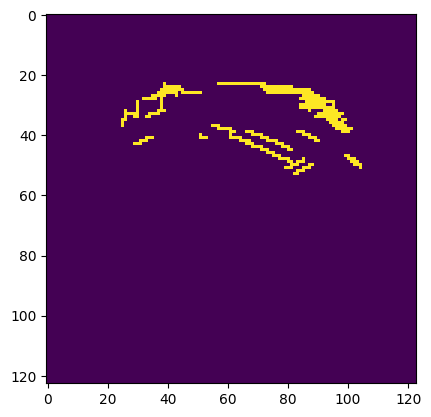
\includegraphics[width=0.5\columnwidth]{img/single_map.png}
% 	\caption{Visualizing a single obstruction map.}
% 	\label{fig:vis-single-map}
% \end{figure}

% Following this approach we can create a simple script to retrieve maps each second and save them locally, later we can export images and create a video to better analyze what is going on. 

% We created a simple script to algorithmically detect handovers, we can use the function \texttt{common.detect\_handovers} to detect whether and handover was performed between two subsequent snaphsots, getting all the handovers is simply a matter of iterating for every JSON file we saved and running the function on each pair.

% We now try to correlate satellite handovers (the vertical dashed lines) with the bandwidth measurements we obtained before, our assumption is we might have drops in bandwidth during handovers. Apparently this does not happen, as we can verify from Figure \ref{fig:vis-correlation-handovers}.

% \begin{figure}
% 	\centering
% 	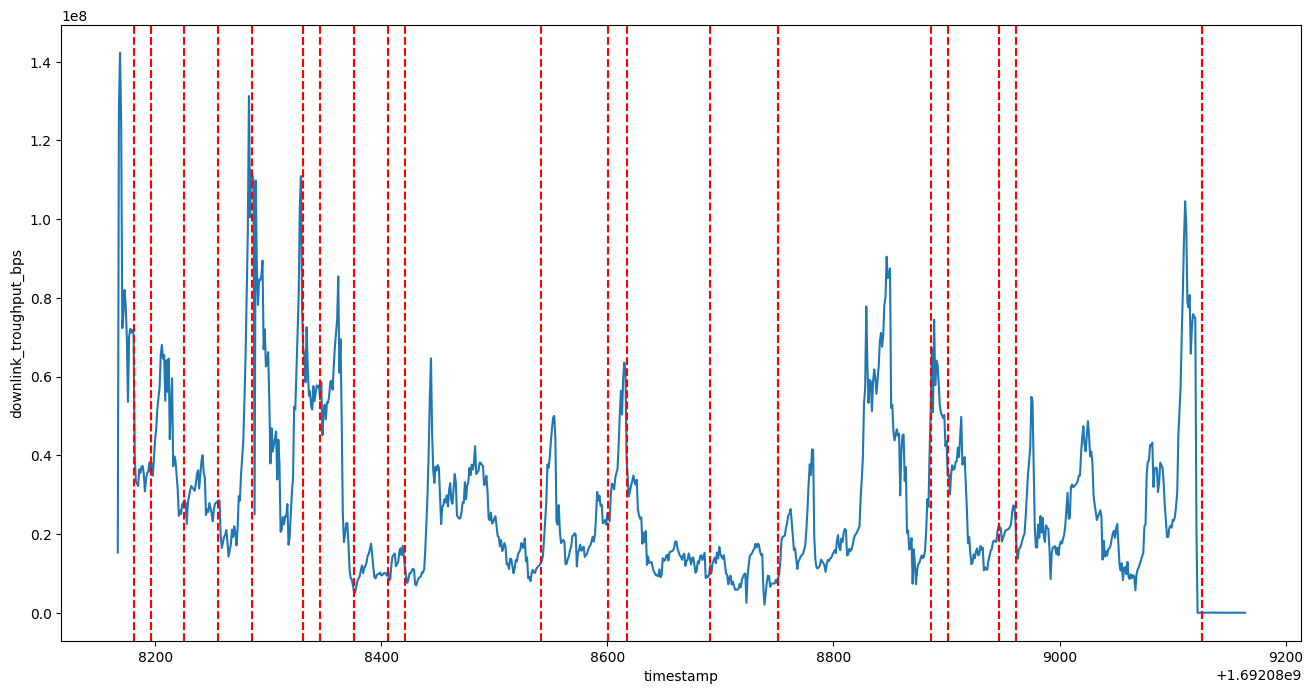
\includegraphics[width=1\columnwidth]{img/correlation_handovers_bw.png}
% 	\caption{Trying to correlate satellite handovers (red vertical lines) with bandwidth measurements.}
% 	\label{fig:vis-correlation-handovers}
% \end{figure}


\chapter{Final Remarks and Future Work}
+ handovers are cool
+ ephemeris
+ project kuiper 

\appendix
\chapter{Appendix}
\label{chap:appendix}


\chapter{Starlink gRPC api}
\label{starlink-grpc}

\subsubsection{\texttt{grpcurl -plaintext 192.168.100.1:9200 describe}}

\begin{lstlisting}[language=bash,basicstyle=\tiny]

rc@gnolmir ~> grpcurl -plaintext 192.168.100.1:9200 describe
SpaceX.API.Device.Device is a service:
service Device {
  rpc Handle ( .SpaceX.API.Device.Request ) returns ( .SpaceX.API.Device.Response );
  rpc Stream ( stream .SpaceX.API.Device.ToDevice ) returns ( stream .SpaceX.API.Device.FromDevice );
}
grpc.reflection.v1alpha.ServerReflection is a service:
service ServerReflection {
  rpc ServerReflectionInfo ( stream .grpc.reflection.v1alpha.ServerReflectionRequest ) returns ( stream .grpc.reflection.v1alpha.ServerReflectionResponse );
}
\end{lstlisting}
\subsubsection{\texttt{grpcurl -plaintext 192.168.100.1:9200 describe SpaceX.API.Device.Request}}

\begin{lstlisting}[language=bash,basicstyle=\tiny]
rc@gnolmir ~> grpcurl -plaintext 192.168.100.1:9200 describe SpaceX.API.Device.Request
SpaceX.API.Device.Request is a message:
message Request {
  uint64 id = 1;
  string target_id = 13;
  uint64 epoch_id = 14;
  oneof request {
    .SpaceX.API.Device.SignedData signed_request = 15;
    .SpaceX.API.Device.RebootRequest reboot = 1001;
    .SpaceX.API.Device.SpeedTestRequest speed_test = 1003;
    .SpaceX.API.Device.GetStatusRequest get_status = 1004;
    .SpaceX.API.Device.AuthenticateRequest authenticate = 1005;
    .SpaceX.API.Device.GetNextIdRequest get_next_id = 1006;
    .SpaceX.API.Device.GetHistoryRequest get_history = 1007;
    .SpaceX.API.Device.GetDeviceInfoRequest get_device_info = 1008;
    .SpaceX.API.Device.GetPingRequest get_ping = 1009;
    .SpaceX.API.Device.SetTrustedKeysRequest set_trusted_keys = 1010;
    .SpaceX.API.Device.FactoryResetRequest factory_reset = 1011;
    .SpaceX.API.Device.GetLogRequest get_log = 1012;
    .SpaceX.API.Device.SetSkuRequest set_sku = 1013;
    .SpaceX.API.Device.UpdateRequest update = 1014;
    .SpaceX.API.Device.GetNetworkInterfacesRequest get_network_interfaces = 1015;
    .SpaceX.API.Device.PingHostRequest ping_host = 1016;
    .SpaceX.API.Device.GetLocationRequest get_location = 1017;
    .SpaceX.API.Device.GetHeapDumpRequest get_heap_dump = 1019;
    .SpaceX.API.Device.RestartControlRequest restart_control = 1020;
    .SpaceX.API.Device.FuseRequest fuse = 1021;
    .SpaceX.API.Device.GetPersistentStatsRequest get_persistent_stats = 1022;
    .SpaceX.API.Device.GetConnectionsRequest get_connections = 1023;
    .SpaceX.API.Device.StartSpeedtestRequest start_speedtest = 1027;
    .SpaceX.API.Device.GetSpeedtestStatusRequest get_speedtest_status = 1028;
    .SpaceX.API.Device.ReportClientSpeedtestRequest report_client_speedtest = 1029;
    .SpaceX.API.Device.InitiateRemoteSshRequest initiate_remote_ssh = 1030 [deprecated = true];
    .SpaceX.API.Device.SelfTestRequest self_test = 1031;
    .SpaceX.API.Device.SetTestModeRequest set_test_mode = 1032;
    .SpaceX.API.Device.SoftwareUpdateRequest software_update = 1033;
    .SpaceX.API.Device.EnableDebugTelemRequest enable_debug_telem = 1034;
    .SpaceX.API.Device.DishStowRequest dish_stow = 2002;
    .SpaceX.API.Device.DishGetContextRequest dish_get_context = 2003;
    .SpaceX.API.Device.DishSetEmcRequest dish_set_emc = 2007;
    .SpaceX.API.Device.DishGetObstructionMapRequest dish_get_obstruction_map = 2008;
    .SpaceX.API.Device.DishGetEmcRequest dish_get_emc = 2009;
    .SpaceX.API.Device.DishSetConfigRequest dish_set_config = 2010;
    .SpaceX.API.Device.DishGetConfigRequest dish_get_config = 2011;
    .SpaceX.API.Device.StartDishSelfTestRequest start_dish_self_test = 2012;
    .SpaceX.API.Device.DishPowerSaveRequest dish_power_save = 2013;
    .SpaceX.API.Device.DishInhibitGpsRequest dish_inhibit_gps = 2014;
    .SpaceX.API.Device.WifiSetConfigRequest wifi_set_config = 3001;
    .SpaceX.API.Device.WifiGetClientsRequest wifi_get_clients = 3002;
    .SpaceX.API.Device.WifiSetupRequest wifi_setup = 3003;
    .SpaceX.API.Device.WifiGetPingMetricsRequest wifi_get_ping_metrics = 3007;
    .SpaceX.API.Device.WifiGetDiagnosticsRequest wifi_get_diagnostics = 3008;
    .SpaceX.API.Device.WifiGetConfigRequest wifi_get_config = 3009;
    .SpaceX.API.Device.WifiSetMeshDeviceTrustRequest wifi_set_mesh_device_trust = 3012;
    .SpaceX.API.Device.WifiSetMeshConfigRequest wifi_set_mesh_config = 3013 [deprecated = true];
    .SpaceX.API.Device.WifiGetClientHistoryRequest wifi_get_client_history = 3015;
    .SpaceX.API.Device.WifiSetAviationConformedRequest wifi_set_aviation_conformed = 3016;
    .SpaceX.API.Device.WifiSetClientGivenNameRequest wifi_set_client_given_name = 3017;
    .SpaceX.API.Device.WifiSelfTestRequest wifi_self_test = 3018;
    .SpaceX.API.Device.TransceiverIFLoopbackTestRequest transceiver_if_loopback_test = 4001;
    .SpaceX.API.Device.TransceiverGetStatusRequest transceiver_get_status = 4003;
    .SpaceX.API.Device.TransceiverGetTelemetryRequest transceiver_get_telemetry = 4004;
  }
  reserved 1018, 1025, 1026, 3011, 3014;
}
\end{lstlisting}

\subsubsection{\texttt{grpcurl -plaintext 192.168.100.1:9200 describe SpaceX.API.Device.Response}}

\begin{lstlisting}[language=bash,basicstyle=\tiny]
rc@gnolmir ~> grpcurl -plaintext 192.168.100.1:9200 describe SpaceX.API.Device.Response
SpaceX.API.Device.Response is a message:
message Response {
  uint64 id = 1;
  .SpaceX.API.Status.Status status = 2;
  uint64 api_version = 3;
  oneof response {
    .SpaceX.API.Device.RebootResponse reboot = 1001;
    .SpaceX.API.Device.SpeedTestResponse speed_test = 1003;
    .SpaceX.API.Device.GetDeviceInfoResponse get_device_info = 1004;
    .SpaceX.API.Device.GetNextIdResponse get_next_id = 1006;
    .SpaceX.API.Device.GetPingResponse get_ping = 1009;
    .SpaceX.API.Device.SetTrustedKeysResponse set_trusted_keys = 1010;
    .SpaceX.API.Device.FactoryResetResponse factory_reset = 1011;
    .SpaceX.API.Device.GetLogResponse get_log = 1012;
    .SpaceX.API.Device.SetSkuResponse set_sku = 1013;
    .SpaceX.API.Device.UpdateResponse update = 1014;
    .SpaceX.API.Device.GetNetworkInterfacesResponse get_network_interfaces = 1015;
    .SpaceX.API.Device.PingHostResponse ping_host = 1016;
    .SpaceX.API.Device.GetLocationResponse get_location = 1017;
    .SpaceX.API.Device.GetHeapDumpResponse get_heap_dump = 1019;
    .SpaceX.API.Device.RestartControlResponse restart_control = 1020;
    .SpaceX.API.Device.FuseResponse fuse = 1021;
    .SpaceX.API.Device.GetConnectionsResponse get_connections = 1023;
    .SpaceX.API.Device.StartSpeedtestResponse start_speedtest = 1027;
    .SpaceX.API.Device.GetSpeedtestStatusResponse get_speedtest_status = 1028;
    .SpaceX.API.Device.ReportClientSpeedtestResponse report_client_speedtest = 1029;
    .SpaceX.API.Device.InitiateRemoteSshResponse initiate_remote_ssh = 1030 [deprecated = true];
    .SpaceX.API.Device.SelfTestResponse self_test = 1031;
    .SpaceX.API.Device.SetTestModeResponse set_test_mode = 1032;
    .SpaceX.API.Device.SoftwareUpdateResponse software_update = 1033;
    .SpaceX.API.Device.EnableDebugTelemResponse enable_debug_telem = 1034;
    .SpaceX.API.Device.DishStowResponse dish_stow = 2002;
    .SpaceX.API.Device.DishGetContextResponse dish_get_context = 2003;
    .SpaceX.API.Device.DishGetStatusResponse dish_get_status = 2004;
    .SpaceX.API.Device.DishAuthenticateResponse dish_authenticate = 2005;
    .SpaceX.API.Device.DishGetHistoryResponse dish_get_history = 2006;
    .SpaceX.API.Device.DishSetEmcResponse dish_set_emc = 2007;
    .SpaceX.API.Device.DishGetObstructionMapResponse dish_get_obstruction_map = 2008;
    .SpaceX.API.Device.DishGetEmcResponse dish_get_emc = 2009;
    .SpaceX.API.Device.DishSetConfigResponse dish_set_config = 2010;
    .SpaceX.API.Device.DishGetConfigResponse dish_get_config = 2011;
    .SpaceX.API.Device.StartDishSelfTestResponse start_dish_self_test = 2012;
    .SpaceX.API.Device.DishInhibitGpsResponse dish_inhibit_gps = 2013;
    .SpaceX.API.Device.WifiSetConfigResponse wifi_set_config = 3001;
    .SpaceX.API.Device.WifiGetClientsResponse wifi_get_clients = 3002;
    .SpaceX.API.Device.WifiSetupResponse wifi_setup = 3003;
    .SpaceX.API.Device.WifiGetStatusResponse wifi_get_status = 3004;
    .SpaceX.API.Device.WifiAuthenticateResponse wifi_authenticate = 3005;
    .SpaceX.API.Device.WifiGetHistoryResponse wifi_get_history = 3006;
    .SpaceX.API.Device.WifiGetPingMetricsResponse wifi_get_ping_metrics = 3007;
    .SpaceX.API.Device.WifiGetDiagnosticsResponse wifi_get_diagnostics = 3008;
    .SpaceX.API.Device.WifiGetConfigResponse wifi_get_config = 3009;
    .SpaceX.API.Device.WifiSetMeshDeviceTrustResponse wifi_set_mesh_device_trust = 3012;
    .SpaceX.API.Device.WifiSetMeshConfigResponse wifi_set_mesh_config = 3013 [deprecated = true];
    .SpaceX.API.Device.WifiGetClientHistoryResponse wifi_get_client_history = 3015;
    .SpaceX.API.Device.WifiSelfTestResponse wifi_self_test = 3016;
    .SpaceX.API.Device.WifiGetPersistentStatsResponse wifi_get_persistent_stats = 3022;
    .SpaceX.API.Device.TransceiverIFLoopbackTestResponse transceiver_if_loopback_test = 4001;
    .SpaceX.API.Device.TransceiverGetStatusResponse transceiver_get_status = 4003;
    .SpaceX.API.Device.TransceiverGetTelemetryResponse transceiver_get_telemetry = 4004;
  }
  reserved 1018, 1026, 2025, 3011, 3014;
}
\end{lstlisting}

\subsubsection{\texttt{grpcurl -plaintext 192.168.100.1:9200 describe SpaceX.API.Device.ToDevice}}

\begin{lstlisting}[language=bash,basicstyle=\tiny]

rc@gnolmir ~ [1]> grpcurl -plaintext 192.168.100.1:9200 describe SpaceX.API.Device.ToDevice
SpaceX.API.Device.ToDevice is a message:
message ToDevice {
  oneof message {
    .SpaceX.API.Device.Request request = 1;
    .SpaceX.API.Device.HealthCheck health_check = 2;
  }
}

\end{lstlisting}

\subsubsection{\texttt{grpcurl -plaintext 192.168.100.1:9200 describe SpaceX.API.Device.FromDevice}}
\begin{lstlisting}[language=bash,basicstyle=\tiny]

rc@gnolmir ~> grpcurl -plaintext 192.168.100.1:9200 describe SpaceX.API.Device.FromDevice
SpaceX.API.Device.FromDevice is a message:
message FromDevice {
  oneof message {
    .SpaceX.API.Device.Response response = 1;
    .SpaceX.API.Device.Event event = 2;
    .SpaceX.API.Device.HealthCheck health_check = 3;
  }
}
\end{lstlisting}



\section{grpcurl requests not working}

\begin{lstlisting}[language=bash,basicstyle=\tiny]

rc@gnolmir:~$ grpcurl -plaintext -d '{"set_test_mode":{}}' 192.168.100.1:9200 SpaceX.API.Device.Device/Handle
ERROR:
  Code: PermissionDenied
  Message: Permission denied
  \end{lstlisting}
\begin{lstlisting}[language=bash,basicstyle=\tiny]

rc@gnolmir:~$ grpcurl -plaintext -d '{"dish_set_config":{}}' 192.168.100.1:9200 SpaceX.API.Device.Device/Handle
ERROR:
  Code: PermissionDenied
  Message: Permission denied
  \end{lstlisting}
\begin{lstlisting}[language=bash,basicstyle=\tiny]

rc@gnolmir:~$ grpcurl -plaintext -d '{"transceiver_if_loopback_test":{}}' 192.168.100.1:9200 SpaceX.API.Device.Device/Handle
ERROR:
  Code: Unimplemented
  Message: Unimplemented
  \end{lstlisting}
\begin{lstlisting}[language=bash,basicstyle=\tiny]

rc@gnolmir:~$ grpcurl -plaintext -d '{"wifi_set_client_given_name":{}}' 192.168.100.1:9200 SpaceX.API.Device.Device/Handle
ERROR:
  Code: Unimplemented
  Message: Unimplemented: *device.Request_WifiSetClientGivenName
  \end{lstlisting}
\begin{lstlisting}[language=bash,basicstyle=\tiny]

rc@gnolmir:~$ grpcurl -plaintext -d '{"wifi_set_aviation_conformed":{}}' 192.168.100.1:9200 SpaceX.API.Device.Device/Handle
ERROR:
  Code: Unimplemented
  Message: Unimplemented: *device.Request_WifiSetAviationConformed
  \end{lstlisting}
\begin{lstlisting}[language=bash,basicstyle=\tiny]

rc@gnolmir:~$ grpcurl -plaintext -d '{"wifi_get_client_history":{}}' 192.168.100.1:9200 SpaceX.API.Device.Device/Handle
ERROR:
  Code: Unimplemented
  Message: Unimplemented: *device.Request_WifiGetClientHistory
  \end{lstlisting}
\begin{lstlisting}[language=bash,basicstyle=\tiny]

rc@gnolmir:~$ grpcurl -plaintext -d '{"wifi_set_mesh_device_trust":{}}' 192.168.100.1:9200 SpaceX.API.Device.Device/Handle
ERROR:
  Code: Unimplemented
  Message: Unimplemented: *device.Request_WifiSetMeshDeviceTrust
  \end{lstlisting}
\begin{lstlisting}[language=bash,basicstyle=\tiny]

rc@gnolmir:~$ grpcurl -plaintext -d '{"wifi_get_ping_metrics":{}}' 192.168.100.1:9200 SpaceX.API.Device.Device/Handle
ERROR:
  Code: Unimplemented
  Message: Unimplemented: *device.Request_WifiGetPingMetrics
  \end{lstlisting}
\begin{lstlisting}[language=bash,basicstyle=\tiny]

rc@gnolmir:~$ grpcurl -plaintext -d '{"wifi_get_diagnostics":{}}' 192.168.100.1:9200 SpaceX.API.Device.Device/Handle
ERROR:
  Code: Unimplemented
  Message: Unimplemented: *device.Request_WifiGetDiagnostics
  \end{lstlisting}
\begin{lstlisting}[language=bash,basicstyle=\tiny]

rc@gnolmir:~$ grpcurl -plaintext -d '{"speed_test":{}}' 192.168.100.1:9200 SpaceX.API.Device.Device/Handle
ERROR:
  Code: Unimplemented
  Message: Unimplemented: *device.Request_SpeedTest
 \end{lstlisting}
\begin{lstlisting}[language=bash,basicstyle=\tiny]

rc@gnolmir:~$ grpcurl -plaintext -d '{"dish_set_emc":{}}' 192.168.100.1:9200 SpaceX.API.Device.Device/Handle
ERROR:
  Code: PermissionDenied
  Message: 
  \end{lstlisting}
\begin{lstlisting}[language=bash,basicstyle=\tiny]

rc@gnolmir:~$ grpcurl -plaintext -d '{"dish_get_emc":{}}' 192.168.100.1:9200 SpaceX.API.Device.Device/Handle
ERROR:
  Code: PermissionDenied
  Message: 
  \end{lstlisting}
\begin{lstlisting}[language=bash,basicstyle=\tiny]

rc@gnolmir:~$ grpcurl -plaintext -d '{"get_persistent_stats":{}}' 192.168.100.1:9200 SpaceX.API.Device.Device/Handle
ERROR:
  Code: Unimplemented
  Message: Unimplemented: *device.Request_GetPersistentStats
\end{lstlisting}
\begin{lstlisting}[language=bash,basicstyle=\tiny]

rc@gnolmir:~$ grpcurl -plaintext -d '{"fuse":{}}' 192.168.100.1:9200 SpaceX.API.Device.Device/Handle
ERROR:
  Code: Unimplemented
  Message: Unimplemented: *device.Request_Fuse
 \end{lstlisting}
 \begin{lstlisting}[language=bash,basicstyle=\tiny]

rc@gnolmir:~$ grpcurl -plaintext -d '{"get_heat_dump":{}}' 192.168.100.1:9200 SpaceX.API.Device.Device/Handle
Error invoking method "SpaceX.API.Device.Device/Handle": error getting request data: message type SpaceX.API.Device.Request has no known field named get_heat_dump
\end{lstlisting}
\begin{lstlisting}[language=bash,basicstyle=\tiny]

rc@gnolmir:~$ grpcurl -plaintext -d '{"set_sku":{}}' 192.168.100.1:9200 SpaceX.API.Device.Device/Handle
ERROR:
  Code: Unimplemented
  Message: Unimplemented: *device.Request_SetSku
 \end{lstlisting}
\begin{lstlisting}[language=bash,basicstyle=\tiny]

rc@gnolmir:~$ grpcurl -plaintext -d '{"update":{}}' 192.168.100.1:9200 SpaceX.API.Device.Device/Handle
ERROR:
  Code: Unimplemented
  Message: Unimplemented: *device.Request_Update
\end{lstlisting}
\begin{lstlisting}[language=bash,basicstyle=\tiny]

rc@gnolmir:~$ grpcurl -plaintext -d '{"authenticate":{}}' 192.168.100.1:9200 SpaceX.API.Device.Device/Handle
ERROR:
  Code: PermissionDenied
  Message: Invalid challenge
\end{lstlisting}
\begin{lstlisting}[language=bash,basicstyle=\tiny]

rc@gnolmir:~$ grpcurl -plaintext -d '{"dish_inibit_gps":{}}' 192.168.100.1:9200 SpaceX.API.Device.Device/Handle
Error invoking method "SpaceX.API.Device.Device/Handle": error getting request data: message type SpaceX.API.Device.Request has no known field named dish_inibit_gps
\end{lstlisting}
\begin{lstlisting}[language=bash,basicstyle=\tiny]

rc@gnolmir:~$ grpcurl -plaintext -d '{"wifi_set_config":{}}' 192.168.100.1:9200 SpaceX.API.Device.Device/Handle
ERROR:
  Code: Unimplemented
  Message: Unimplemented: *device.Request_WifiSetConfig
\end{lstlisting}
\begin{lstlisting}[language=bash,basicstyle=\tiny]

rc@gnolmir:~$ grpcurl -plaintext -d '{"wifi_get_config":{}}' 192.168.100.1:9200 SpaceX.API.Device.Device/Handle
ERROR:
  Code: Unimplemented
  Message: Unimplemented: *device.Request_WifiGetConfig
\end{lstlisting}
\begin{lstlisting}[language=bash,basicstyle=\tiny]

rc@gnolmir:~$ grpcurl -plaintext -d '{"wifi_get_config":{}}' 192.168.100.1:9200 SpaceX.API.Device.Device/Handle
ERROR:
  Code: Unimplemented
  Message: Unimplemented: *device.Request_WifiGetConfig
\end{lstlisting}
\begin{lstlisting}[language=bash,basicstyle=\tiny]
 
rc@gnolmir:~$ grpcurl -plaintext -d '{"get_ping":{}}' 192.168.100.1:9200 SpaceX.API.Device.Device/Handle
ERROR:
  Code: Unimplemented
  Message: Unimplemented: *device.Request_GetPing
\end{lstlisting}

\begin{lstlisting}[language=bash,basicstyle=\tiny]
rc@gnolmir:~$ grpcurl -plaintext  -d '{"restart_control":{}}' 192.168.100.1:9200 SpaceX.API.Device.Device/Handle
ERROR:
  Code: Unimplemented
  Message: Unimplemented: *device.Request_RestartControl
\end{lstlisting}

\begin{lstlisting}[language=bash,basicstyle=\tiny]x
rc@gnolmir:~$ grpcurl -plaintext -d '{"get_log":{}}' 192.168.100.1:9200 SpaceX.API.Device.Device/Handle
ERROR:
  Code: Unimplemented
  Message: Unimplemented: *device.Request_GetLog
\end{lstlisting}

\begin{lstlisting}[language=bash,basicstyle=\tiny]
rc@gnolmir:~$ grpcurl -plaintext -d '{"get_network_interfaces":{}}' 192.168.100.1:9200 SpaceX.API.Device.Device/Handle
ERROR:
  Code: Unimplemented
  Message: Unimplemented: *device.Request_GetNetworkInterfaces
\end{lstlisting}

\begin{lstlisting}[language=bash,basicstyle=\tiny]
rc@gnolmir:~$ grpcurl -plaintext -d '{"ping_host":{}}' 192.168.100.1:9200 SpaceX.API.Device.Device/Handle
ERROR:
  Code: Unimplemented
  Message: Unimplemented: *device.Request_PingHost
\end{lstlisting}

\begin{lstlisting}[language=bash,basicstyle=\tiny]
rc@gnolmir:~$ grpcurl -plaintext -d '{"enable_debug_telem":{}}' 192.168.100.1:9200 SpaceX.API.Device.Device/Handle
ERROR:
  Code: Unimplemented
  Message: Unimplemented: *device.Request_EnableDebugTelem
\end{lstlisting}

\begin{lstlisting}[language=bash,basicstyle=\tiny]
rc@gnolmir:~$ grpcurl -plaintext -d '{"wifi_get_clients":{}}' 192.168.100.1:9200 SpaceX.API.Device.Device/Handle
ERROR:
  Code: Unimplemented
  Message: Unimplemented: *device.Request_WifiGetClients
\end{lstlisting}

\begin{lstlisting}[language=bash,basicstyle=\tiny]
rc@gnolmir:~$ grpcurl -plaintext -d '{"wifi_setup":{}}' 192.168.100.1:9200 SpaceX.API.Device.Device/Handle
ERROR:
  Code: Unimplemented
  Message: Unimplemented: *device.Request_WifiSetup
\end{lstlisting}

\begin{lstlisting}[language=bash,basicstyle=\tiny]
rc@gnolmir:~$ grpcurl -plaintext -d '{"transceiver_get_telemetry":{}}' 192.168.100.1:9200 SpaceX.API.Device.Device/Handle
ERROR:
  Code: Unimplemented
  Message: Unimplemented
\end{lstlisting}

\begin{lstlisting}[language=bash,basicstyle=\tiny]
rc@gnolmir:~$ grpcurl -plaintext -d '{"get_connections":{}}' 192.168.100.1:9200 SpaceX.API.Device.Device/Handle
ERROR:
  Code: Unimplemented
  Message: Unimplemented: *device.Request_GetConnections
\end{lstlisting}

\begin{lstlisting}[language=bash,basicstyle=\tiny]
rc@gnolmir:~$ grpcurl -plaintext -d '{"get_next_id":{}}' 192.168.100.1:9200 SpaceX.API.Device.Device/Handle
ERROR:
  Code: Unimplemented
  Message: Unimplemented: *device.Request_GetNextId
\end{lstlisting}

\begin{lstlisting}[language=bash,basicstyle=\tiny]
rc@gnolmir:~$ grpcurl -plaintext -d '{"speed_test":{}}' 192.168.100.1:9200 SpaceX.API.Device.Device/Handle
ERROR:
  Code: Unimplemented
  Message: Unimplemented: *device.Request_SpeedTest
\end{lstlisting}
\begin{lstlisting}[language=bash,basicstyle=\tiny]
  
rc@gnolmir:~$ grpcurl -plaintext -d '{"get_ping":{}}' 192.168.100.1:9200 SpaceX.API.Device.Device/Handle
ERROR:
  Code: Unimplemented
  Message: Unimplemented: *device.Request_GetPing
\end{lstlisting}
\begin{lstlisting}[language=bash,basicstyle=\tiny]

rc@gnolmir:~$ grpcurl -plaintext -d '{"get_network_interfaces":{}}' 192.168.100.1:9200 SpaceX.API.Device.Device/Handle
ERROR:
  Code: Unimplemented
  Message: Unimplemented: *device.Request_GetNetworkInterfaces
\end{lstlisting}

\begin{lstlisting}[language=bash,basicstyle=\tiny]

rc@gnolmir:~$ grpcurl -plaintext -d '{"transceiver_get_telemetry":{}}' 192.168.100.1:9200 SpaceX.API.Device.Device/Handle
ERROR:
  Code: Unimplemented
  Message: Unimplemented
\end{lstlisting}
\begin{lstlisting}[language=bash,basicstyle=\tiny]

rc@gnolmir:~$ grpcurl -plaintext -d '{"transceiver_get_status":{}}' 192.168.100.1:9200 SpaceX.API.Device.Device/Handle
ERROR:
  Code: Unimplemented
  Message: Unimplemented
\end{lstlisting}
\begin{lstlisting}[language=bash,basicstyle=\tiny]

rc@gnolmir:~$ grpcurl -plaintext -d '{"get_location":{}}' 192.168.100.1:9200 SpaceX.API.Device.Device/Handle
ERROR:
  Code: PermissionDenied
  Message: GetLocation requests are not enabled on this device
\end{lstlisting}
\begin{lstlisting}[language=bash,basicstyle=\tiny]

rc@gnolmir:~$ grpcurl -plaintext -d '{"dish_get_context":{}}' 192.168.100.1:9200 SpaceX.API.Device.Device/Handle
ERROR:
  Code: PermissionDenied
  Message: Permission denied
\end{lstlisting}
\begin{lstlisting}[language=bash,basicstyle=\tiny]

rc@gnolmir:~$ grpcurl -plaintext -d '{"software_update":{}}' 192.168.100.1:9200 SpaceX.API.Device.Device/Handle
ERROR:
  Code: FailedPrecondition
  Message: Software update stream not open
\end{lstlisting}


\section{grpcurl requests  working}
\begin{lstlisting}[language=bash,basicstyle=\tiny]

rc@gnolmir:~$ grpcurl -plaintext -d '{"reboot":{}}' 192.168.100.1:9200 SpaceX.API.Device.Device/Handle
{
  "apiVersion": "8",
  "reboot": {
    
  }
}
\end{lstlisting}
\begin{lstlisting}[language=bash,basicstyle=\tiny]

rc@gnolmir:~$ grpcurl -plaintext -d '{"get_status":{}}' 192.168.100.1:9200 SpaceX.API.Device.Device/Handle
{
  "apiVersion": "8",
  "dishGetStatus": {
    "deviceInfo": {
      "id": "ut01000000-00000000-00270e41",
      "hardwareVersion": "rev3_proto2",
      "softwareVersion": "2ce8c16a-67b6-4bbd-a135-a00662a60151.uterm.release",
      "countryCode": "DE",
      "utcOffsetS": 1,
      "bootcount": 69,
      "generationNumber": "1684883829"
    },
    "deviceState": {
      "uptimeS": "628401"
    },
    "obstructionStats": {
      "validS": 628111,
      "avgProlongedObstructionIntervalS": "NaN",
      "timeObstructed": 6.3682954e-08,
      "patchesValid": 4097
    },
    "alerts": {
      
    },
    "downlinkThroughputBps": 20560.479,
    "uplinkThroughputBps": 9042.919,
    "popPingLatencyMs": 34.52381,
    "boresightAzimuthDeg": 1.6949656,
    "boresightElevationDeg": 63.424454,
    "gpsStats": {
      "gpsValid": true,
      "gpsSats": 10
    },
    "ethSpeedMbps": 1000,
    "mobilityClass": "MOBILE",
    "isSnrAboveNoiseFloor": true,
    "readyStates": {
      "cady": true,
      "scp": true,
      "l1l2": true,
      "xphy": true,
      "aap": true,
      "rf": true
    },
    "softwareUpdateState": "IDLE",
    "disablementCode": "OKAY",
    "softwareUpdateStats": {
      "softwareUpdateState": "IDLE",
      "softwareUpdateProgress": 1
    },
    "alignmentStats": {
      "tiltAngleDeg": 26.285408,
      "boresightAzimuthDeg": 1.6949656,
      "boresightElevationDeg": 63.424454,
      "attitudeEstimationState": "FILTER_CONVERGED",
      "attitudeUncertaintyDeg": 0.53231573
    },
    "initializationDurationSeconds": {
      "attitudeInitialization": 112,
      "burstDetected": 36,
      "ekfConverged": 155,
      "firstCplane": 63,
      "firstPopPing": 72,
      "gpsValid": 28,
      "initialNetworkEntry": 36,
      "networkSchedule": 68,
      "rfReady": 34,
      "stableConnection": 113
    },
    "config": {
      "powerSaveDurationMinutes": 1,
      "applySnowMeltMode": true,
      "applyLocationRequestMode": true,
      "applyLevelDishMode": true,
      "applyPowerSaveStartMinutes": true,
      "applyPowerSaveDurationMinutes": true,
      "applyPowerSaveMode": true
    }
  }
}
\end{lstlisting}

\begin{lstlisting}[language=bash,basicstyle=\tiny]

rc@gnolmir:~$ grpcurl -plaintext -d '{"start_dish_self_test":{}}' 192.168.100.1:9200 SpaceX.API.Device.Device/Handle
{
  "apiVersion": "8",
  "startDishSelfTest": {
    
  }
}
\end{lstlisting}
\begin{lstlisting}[language=bash,basicstyle=\tiny]

rc@gnolmir:~$ grpcurl -plaintext -d '{"get_history":{}}' 192.168.100.1:9200 SpaceX.API.Device.Device/Handle
{
  "apiVersion": "8",
  "dishGetHistory": {
    "current": "626676",
    "popPingDropRate": [0,0,...,0,0],
    "popPingLatencyMs": [48.333332,47.8,...,46.666668,47.47619],
    "downlinkThroughputBps": [14705.2295,24805.113,...,6928.99,9714.008],
    "uplinkThroughputBps": [17733.518,11911.823,...,9042.919,34309.406],
    "outages": [
      {
        "cause": "NO_DOWNLINK",
        "startTimestampNs": "1371246075160167224",
        "durationNs": "400011278",
        "didSwitch": true
      },
      {
        "cause": "NO_PINGS",
        "startTimestampNs": "1371283269140157964",
        "durationNs": "999988759",
        "didSwitch": true
      }
    ....
    ]
  }
}
\end{lstlisting}
\begin{lstlisting}[language=bash,basicstyle=\tiny]

rc@gnolmir:~$ grpcurl -plaintext -d '{"get_device_info":{}}' 192.168.100.1:9200 SpaceX.API.Device.Device/Handle
{
  "apiVersion": "8",
  "getDeviceInfo": {
    "deviceInfo": {
      "id": "ut01000000-00000000-00270e41",
      "hardwareVersion": "rev3_proto2",
      "softwareVersion": "2ce8c16a-67b6-4bbd-a135-a00662a60151.uterm.release",
      "countryCode": "DE",
      "utcOffsetS": 1,
      "bootcount": 69,
      "generationNumber": "1684883829"
    }
  }
}
\end{lstlisting}

\begin{lstlisting}[language=bash,basicstyle=\tiny]

rc@gnolmir:~$ grpcurl -plaintext  -d '{"dish_power_save":{"power_save_duration_minutes":1}}' 192.168.100.1:9200 SpaceX.API.Device.Device/Handle
{
  "status": {
    
  },
  "apiVersion": "8"
}
\end{lstlisting}
\begin{lstlisting}[language=bash,basicstyle=\tiny]

rc@gnolmir:~$ grpcurl -plaintext -d '{"dish_get_config":{}}' 192.168.100.1:9200 SpaceX.API.Device.Device/Handle
{
  "apiVersion": "8",
  "dishGetConfig": {
    "dishConfig": {
      "powerSaveDurationMinutes": 1,
      "applySnowMeltMode": true,
      "applyLocationRequestMode": true,
      "applyLevelDishMode": true,
      "applyPowerSaveStartMinutes": true,
      "applyPowerSaveDurationMinutes": true,
      "applyPowerSaveMode": true
    }
  }
}
\end{lstlisting}
\begin{lstlisting}[language=bash,basicstyle=\tiny]

rc@gnolmir:~$ grpcurl -plaintext -d '{"dish_get_obstruction_map":{}}' 192.168.100.1:9200 SpaceX.API.Device.Device/Handle
(output omitted)
\end{lstlisting}
% \section{Appendix section}

\begin{lstlisting}[language=python,caption={the \texttt{calculate\_visible\_satellites} function},captionpos=b]
def calculate_visible_satellites(
    observer_latitude, observer_longitude, observer_elevation, distance_km
):
    stations_url = "https://celestrak.org/NORAD/elements/gp.php?GROUP=starlink&FORMAT=tle"

    satellites = load.tle_file(stations_url)
    observer = Topos(observer_latitude, observer_longitude, observer_elevation)
    ts = load.timescale()
    t = ts.now()

    # Calculate satellite positions
    positions = []
    for sat in satellites:
        satellite = sat
        position = (satellite - observer).at(t)
        positions.append((sat, position))

    # Filter visible satellites
    visible_satellites = []
    for sat, position in positions:
        alt, az, distance = position.altaz()
        # Satellite is above the horizon
        if alt.degrees > 0 and distance.km < distance_km:
            visible_satellites.append((sat, alt, az))

    return visible_satellites
\end{lstlisting}

\chapter{Skyfield Library}
\label{app:sky}
\begin{lstlisting}[language=python,caption={retrieving a Satellite's position using the Satname},captionpos=b]
from skyfield.api import load, wgs84

stations_url = "https://celestrak.org/NORAD/elements/gp.php?GROUP=starlink&FORMAT=tle"
satellites = load.tle_file(stations_url)
print("Loaded", len(satellites), "satellites")
by_name = {sat.name: sat for sat in satellites}
satellite = by_name["STARLINK-1007"]

# year, month, day, hour, minute, second
ts = load.timescale()
t = ts.now()
a = satellite.at(t)
lat, lon = wgs84.latlon_of(a)
print("Latitude:", lat)
print("Longitude:", lon)
\end{lstlisting}



\clearpage
\pagestyle{thesischapter}
\cleardoublepage
\selectlanguage{english}
\printbibliography[heading=bibintoc]
\clearpage
\pagestyle{empty}
\end{document}
